% inspired from http://tex.stackexchange.com/questions/56611/make-a-vigen%C3%A8re-rectangular-in-latex
\documentclass{article}

\usepackage{tikz}
\usetikzlibrary{positioning}

\begin{document}

% Exemple d'utilisation du chiffre de César

% Chiffrement

% tour 1
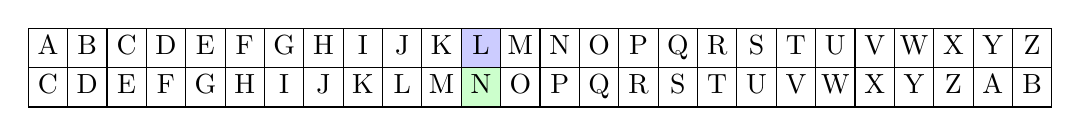
\begin{tikzpicture}
   \foreach \i in {0,...,10} {
      \node[draw, minimum size = 0.5cm, inner sep = 0pt]
      at (\i*0.5,0) {\strut\symbol{\numexpr`A+\i\relax}};
   }
   \foreach \i in {11,...,11} {
      \node[draw, minimum size = 0.5cm, inner sep = 0pt, fill = blue!20]
      at (\i*0.5,0) {\strut\symbol{\numexpr`A+\i\relax}};
   }
   \foreach \i in {12,...,25} {
      \node[draw, minimum size = 0.5cm, inner sep = 0pt]
      at (\i*0.5,0) {\strut\symbol{\numexpr`A+\i\relax}};
   }

   \foreach \i in {0,...,10} {
      \foreach \j in {2,...,2} {
         \edef\k{\ifnum\numexpr\i+\j\relax>25
            \the\numexpr\i+\j-26\relax
            \else
            \the\numexpr\i+\j\relax
         \fi}
         \node[draw, minimum size = 0.5cm, inner sep = 0pt]
         at (\i*0.5,-0.5) {\strut\symbol{\numexpr`A+\k\relax}};
      }
   }
   \foreach \i in {11,...,11} {
      \foreach \j in {2,...,2} {
         \edef\k{\ifnum\numexpr\i+\j\relax>25
            \the\numexpr\i+\j-26\relax
            \else
            \the\numexpr\i+\j\relax
         \fi}
         \node[draw, minimum size = 0.5cm, inner sep = 0pt, fill = green!20]
         at (\i*0.5,-0.5) {\strut\symbol{\numexpr`A+\k\relax}};
      }
   }
   \foreach \i in {12,...,25} {
      \foreach \j in {2,...,2} {
         \edef\k{\ifnum\numexpr\i+\j\relax>25
            \the\numexpr\i+\j-26\relax
            \else
            \the\numexpr\i+\j\relax
         \fi}
         \node[draw, minimum size = 0.5cm, inner sep = 0pt]
         at (\i*0.5,-0.5) {\strut\symbol{\numexpr`A+\k\relax}};
      }
   }

\end{tikzpicture}

\vspace{0.5cm}

\begin{tikzpicture}
   \node [anchor = center] (first) {N};
\end{tikzpicture}

% tour 2

\vspace{1cm}

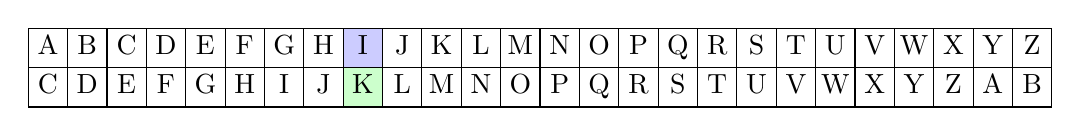
\begin{tikzpicture}
   \foreach \i in {0,...,7} {
      \node[draw, minimum size = 0.5cm, inner sep = 0pt]
      at (\i*0.5,0) {\strut\symbol{\numexpr`A+\i\relax}};
   }
   \foreach \i in {8,...,8} {
      \node[draw, minimum size = 0.5cm, inner sep = 0pt, fill = blue!20]
      at (\i*0.5,0) {\strut\symbol{\numexpr`A+\i\relax}};
   }
   \foreach \i in {9,...,25} {
      \node[draw, minimum size = 0.5cm, inner sep = 0pt]
      at (\i*0.5,0) {\strut\symbol{\numexpr`A+\i\relax}};
   }

   \foreach \i in {0,...,7} {
      \foreach \j in {2,...,2} {
         \edef\k{\ifnum\numexpr\i+\j\relax>25
            \the\numexpr\i+\j-26\relax
            \else
            \the\numexpr\i+\j\relax
         \fi}
         \node[draw, minimum size = 0.5cm, inner sep = 0pt]
         at (\i*0.5,-0.5) {\strut\symbol{\numexpr`A+\k\relax}};
      }
   }
   \foreach \i in {8,...,8} {
      \foreach \j in {2,...,2} {
         \edef\k{\ifnum\numexpr\i+\j\relax>25
            \the\numexpr\i+\j-26\relax
            \else
            \the\numexpr\i+\j\relax
         \fi}
         \node[draw, minimum size = 0.5cm, inner sep = 0pt, fill = green!20]
         at (\i*0.5,-0.5) {\strut\symbol{\numexpr`A+\k\relax}};
      }
   }
   \foreach \i in {9,...,25} {
      \foreach \j in {2,...,2} {
         \edef\k{\ifnum\numexpr\i+\j\relax>25
            \the\numexpr\i+\j-26\relax
            \else
            \the\numexpr\i+\j\relax
         \fi}
         \node[draw, minimum size = 0.5cm, inner sep = 0pt]
         at (\i*0.5,-0.5) {\strut\symbol{\numexpr`A+\k\relax}};
      }
   }

\end{tikzpicture}

\vspace{0.5cm}


\begin{tikzpicture}
   \node [anchor = center] (first) {N};
   \node [anchor = center, right = 0cm of first] (second) {K};
\end{tikzpicture}

% tour 3

\vspace{1cm}

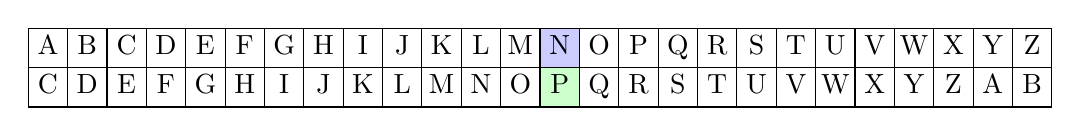
\begin{tikzpicture}
   \foreach \i in {0,...,12} {
      \node[draw, minimum size = 0.5cm, inner sep = 0pt]
      at (\i*0.5,0) {\strut\symbol{\numexpr`A+\i\relax}};
   }
   \foreach \i in {13,...,13} {
      \node[draw, minimum size = 0.5cm, inner sep = 0pt, fill = blue!20]
      at (\i*0.5,0) {\strut\symbol{\numexpr`A+\i\relax}};
   }
   \foreach \i in {14,...,25} {
      \node[draw, minimum size = 0.5cm, inner sep = 0pt]
      at (\i*0.5,0) {\strut\symbol{\numexpr`A+\i\relax}};
   }

   \foreach \i in {0,...,12} {
      \foreach \j in {2,...,2} {
         \edef\k{\ifnum\numexpr\i+\j\relax>25
            \the\numexpr\i+\j-26\relax
            \else
            \the\numexpr\i+\j\relax
         \fi}
         \node[draw, minimum size = 0.5cm, inner sep = 0pt]
         at (\i*0.5,-0.5) {\strut\symbol{\numexpr`A+\k\relax}};
      }
   }
   \foreach \i in {13,...,13} {
      \foreach \j in {2,...,2} {
         \edef\k{\ifnum\numexpr\i+\j\relax>25
            \the\numexpr\i+\j-26\relax
            \else
            \the\numexpr\i+\j\relax
         \fi}
         \node[draw, minimum size = 0.5cm, inner sep = 0pt, fill = green!20]
         at (\i*0.5,-0.5) {\strut\symbol{\numexpr`A+\k\relax}};
      }
   }
   \foreach \i in {14,...,25} {
      \foreach \j in {2,...,2} {
         \edef\k{\ifnum\numexpr\i+\j\relax>25
            \the\numexpr\i+\j-26\relax
            \else
            \the\numexpr\i+\j\relax
         \fi}
         \node[draw, minimum size = 0.5cm, inner sep = 0pt]
         at (\i*0.5,-0.5) {\strut\symbol{\numexpr`A+\k\relax}};
      }
   }

\end{tikzpicture}

\vspace{0.5cm}


\begin{tikzpicture}
   \node [anchor = center] (first) {N};
   \node [anchor = center, right = 0cm of first] (second) {K};
   \node [anchor = center, right = 0cm of second] (third) {P};
\end{tikzpicture}

\vspace{0.5cm}

\begin{tikzpicture}
   \node [anchor = center] (first) {...};
\end{tikzpicture}

\vspace{0.5cm}


\begin{tikzpicture}
   \node [anchor = center] (first) {N};
   \node [anchor = center, right = 0cm of first] (second) {K};
   \node [anchor = center, right = 0cm of second] (third) {P};
   \node [anchor = center, right = 0cm of third] (fourth) {W};
   \node [anchor = center, right = 0cm of fourth] (fifth) {Z};
\end{tikzpicture}

% Déchiffrement

\newpage

% tour 1
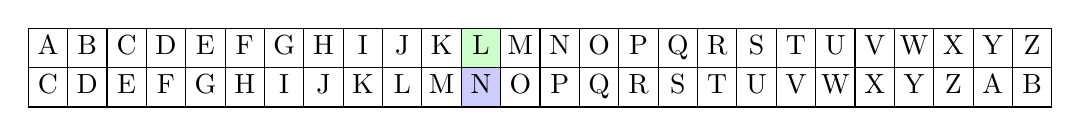
\begin{tikzpicture}
   \foreach \i in {0,...,10} {
      \node[draw, minimum size = 0.5cm, inner sep = 0pt]
      at (\i*0.5,0) {\strut\symbol{\numexpr`A+\i\relax}};
   }
   \foreach \i in {11,...,11} {
      \node[draw, minimum size = 0.5cm, inner sep = 0pt, fill = green!20]
      at (\i*0.5,0) {\strut\symbol{\numexpr`A+\i\relax}};
   }
   \foreach \i in {12,...,25} {
      \node[draw, minimum size = 0.5cm, inner sep = 0pt]
      at (\i*0.5,0) {\strut\symbol{\numexpr`A+\i\relax}};
   }

   \foreach \i in {0,...,10} {
      \foreach \j in {2,...,2} {
         \edef\k{\ifnum\numexpr\i+\j\relax>25
            \the\numexpr\i+\j-26\relax
            \else
            \the\numexpr\i+\j\relax
         \fi}
         \node[draw, minimum size = 0.5cm, inner sep = 0pt]
         at (\i*0.5,-0.5) {\strut\symbol{\numexpr`A+\k\relax}};
      }
   }
   \foreach \i in {11,...,11} {
      \foreach \j in {2,...,2} {
         \edef\k{\ifnum\numexpr\i+\j\relax>25
            \the\numexpr\i+\j-26\relax
            \else
            \the\numexpr\i+\j\relax
         \fi}
         \node[draw, minimum size = 0.5cm, inner sep = 0pt, fill = blue!20]
         at (\i*0.5,-0.5) {\strut\symbol{\numexpr`A+\k\relax}};
      }
   }
   \foreach \i in {12,...,25} {
      \foreach \j in {2,...,2} {
         \edef\k{\ifnum\numexpr\i+\j\relax>25
            \the\numexpr\i+\j-26\relax
            \else
            \the\numexpr\i+\j\relax
         \fi}
         \node[draw, minimum size = 0.5cm, inner sep = 0pt]
         at (\i*0.5,-0.5) {\strut\symbol{\numexpr`A+\k\relax}};
      }
   }

\end{tikzpicture}

\vspace{0.5cm}

\begin{tikzpicture}
   \node [anchor = center] (first) {L};
\end{tikzpicture}

% tour 2

\vspace{1cm}

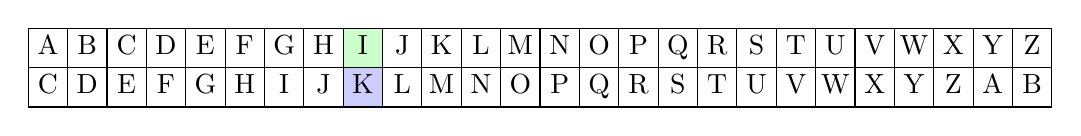
\begin{tikzpicture}
   \foreach \i in {0,...,7} {
      \node[draw, minimum size = 0.5cm, inner sep = 0pt]
      at (\i*0.5,0) {\strut\symbol{\numexpr`A+\i\relax}};
   }
   \foreach \i in {8,...,8} {
      \node[draw, minimum size = 0.5cm, inner sep = 0pt, fill = green!20]
      at (\i*0.5,0) {\strut\symbol{\numexpr`A+\i\relax}};
   }
   \foreach \i in {9,...,25} {
      \node[draw, minimum size = 0.5cm, inner sep = 0pt]
      at (\i*0.5,0) {\strut\symbol{\numexpr`A+\i\relax}};
   }

   \foreach \i in {0,...,7} {
      \foreach \j in {2,...,2} {
         \edef\k{\ifnum\numexpr\i+\j\relax>25
            \the\numexpr\i+\j-26\relax
            \else
            \the\numexpr\i+\j\relax
         \fi}
         \node[draw, minimum size = 0.5cm, inner sep = 0pt]
         at (\i*0.5,-0.5) {\strut\symbol{\numexpr`A+\k\relax}};
      }
   }
   \foreach \i in {8,...,8} {
      \foreach \j in {2,...,2} {
         \edef\k{\ifnum\numexpr\i+\j\relax>25
            \the\numexpr\i+\j-26\relax
            \else
            \the\numexpr\i+\j\relax
         \fi}
         \node[draw, minimum size = 0.5cm, inner sep = 0pt, fill = blue!20]
         at (\i*0.5,-0.5) {\strut\symbol{\numexpr`A+\k\relax}};
      }
   }
   \foreach \i in {9,...,25} {
      \foreach \j in {2,...,2} {
         \edef\k{\ifnum\numexpr\i+\j\relax>25
            \the\numexpr\i+\j-26\relax
            \else
            \the\numexpr\i+\j\relax
         \fi}
         \node[draw, minimum size = 0.5cm, inner sep = 0pt]
         at (\i*0.5,-0.5) {\strut\symbol{\numexpr`A+\k\relax}};
      }
   }

\end{tikzpicture}

\vspace{0.5cm}

\begin{tikzpicture}
   \node [anchor = center] (first) {L};
   \node [anchor = center, right = 0cm of first] (second) {I};
\end{tikzpicture}

% tour 3

\vspace{1cm}

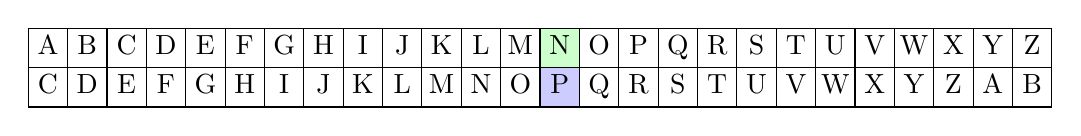
\begin{tikzpicture}
   \foreach \i in {0,...,12} {
      \node[draw, minimum size = 0.5cm, inner sep = 0pt]
      at (\i*0.5,0) {\strut\symbol{\numexpr`A+\i\relax}};
   }
   \foreach \i in {13,...,13} {
      \node[draw, minimum size = 0.5cm, inner sep = 0pt, fill = green!20]
      at (\i*0.5,0) {\strut\symbol{\numexpr`A+\i\relax}};
   }
   \foreach \i in {14,...,25} {
      \node[draw, minimum size = 0.5cm, inner sep = 0pt]
      at (\i*0.5,0) {\strut\symbol{\numexpr`A+\i\relax}};
   }

   \foreach \i in {0,...,12} {
      \foreach \j in {2,...,2} {
         \edef\k{\ifnum\numexpr\i+\j\relax>25
            \the\numexpr\i+\j-26\relax
            \else
            \the\numexpr\i+\j\relax
         \fi}
         \node[draw, minimum size = 0.5cm, inner sep = 0pt]
         at (\i*0.5,-0.5) {\strut\symbol{\numexpr`A+\k\relax}};
      }
   }
   \foreach \i in {13,...,13} {
      \foreach \j in {2,...,2} {
         \edef\k{\ifnum\numexpr\i+\j\relax>25
            \the\numexpr\i+\j-26\relax
            \else
            \the\numexpr\i+\j\relax
         \fi}
         \node[draw, minimum size = 0.5cm, inner sep = 0pt, fill = blue!20]
         at (\i*0.5,-0.5) {\strut\symbol{\numexpr`A+\k\relax}};
      }
   }
   \foreach \i in {14,...,25} {
      \foreach \j in {2,...,2} {
         \edef\k{\ifnum\numexpr\i+\j\relax>25
            \the\numexpr\i+\j-26\relax
            \else
            \the\numexpr\i+\j\relax
         \fi}
         \node[draw, minimum size = 0.5cm, inner sep = 0pt]
         at (\i*0.5,-0.5) {\strut\symbol{\numexpr`A+\k\relax}};
      }
   }

\end{tikzpicture}

\vspace{0.5cm}


\begin{tikzpicture}
   \node [anchor = center] (first) {L};
   \node [anchor = center, right = 0cm of first] (second) {I};
   \node [anchor = center, right = 0cm of second] (third) {N};
\end{tikzpicture}

\vspace{0.5cm}

\begin{tikzpicture}
   \node [anchor = center] (first) {...};
\end{tikzpicture}

\vspace{0.5cm}


\begin{tikzpicture}
   \node [anchor = center] (first) {L};
   \node [anchor = center, right = 0cm of first] (second) {I};
   \node [anchor = center, right = 0cm of second] (third) {N};
   \node [anchor = center, right = 0cm of third] (fourth) {U};
   \node [anchor = center, right = 0cm of fourth] (fifth) {X};
\end{tikzpicture}

\end{document}
